\chapter{Discussion}\label{chapter:discussion}

\section{Benefits of fast traders}

\subsection{Fast market makers reduce price flickering}
In 


\section{Agent strategies market crashes}


It is somewhat intuitive that HFT chartists should be suspected of having an influence on the market such that the market become more likely to crash. The results did indeed confirm this, as it was shown that a negative correlation exists between the number of chartists active in the market, and the size of the overshoot (see figure \ref{fig:d11_parvfit_scAgents}). 

It is conceivable that the market makers also contribute to the market crashing, since the market makers also ignore the true fundamental price. Indeed, the results showed that the market does not crash from having fast chartists alone. The results also showed that the market will not crash from having only fast market makers either. Instead, both types of fast traders were required to make the market crash. The following text will provide an explanation as to why this is so.

It was found that markets containing no market makers will almost never crash. Without the presence of market makers, even a market saturated with chartists will eventually return to the fundamental price, as the force of the initial downtrend created by the fundamentalists dissipates. 


\subsubsection*{Case with no fast traders}
The shock to the fundamental creates a drive in the market for falling prices, due to the presence of the fundamentalists. The fundamentalists have a large delay, and the downwards drive is therefore initially small, as most of the fundamentalists fail to observe that the shock has happened. As the fundamentalists begin to observe the shock, they start submitting sell orders at lower prices, as they believe that the stock is no longer worth the price at which they were previously willing to sell. Hence, the number of sell orders starts to increase. 

As for the buy side of the order book, the number of new buy orders starts to fall, as the fundamentalists start to register the shock. The buy orders that were previously submitted by slow traders at prices slightly below the old fundamental are not canceled, as the model assumes that the fundamentalists are too slow to register the change in the fundamental. Furthermore, in order to simulate an order book with a long trade history, the order book was initialized with a large number of market orders with a normal price distribution centered around the initial fundamental. These buy orders provide matches for the increasing number of sell orders, and the traded price begins to drop. If the market has no fast traders, the traded price will eventually reach the new fundamental, and stay within the stability margin. Thus, in the rather simple case where the market only contains fundamentalists, crashes do not occur. 

\subsubsection*{Case with chartists but no market makers}
When adding chartists, the market starts to behave in a different manner. The chartists do not use any information about the true true fundamental price, but are instead only concerned with the actual traded price. After the shock, the fundamentalists start submitting bids to sell at lower prices, Depending on the parameters of the chartists, some chartists will interpret this as a downtrend, while others will not. The chartists that detect a downtrend will start submitting bids to sell at a lower price, as they believe the price will continue to drop. The chartists that did not detect a trend will remain inactive. The sell orders submitted by  the chartists are matched by previously existing buy market orders at lower prices. Hence, the chartists add to the force that drives the traded price down by submitting sell orders at lower prices. However, since the only active traders in the market are fundamentalists and chartists, the supply of buy orders at prices lower than the new fundamental are limited. The chartists that detected a downtrend will exclusively place sell orders, and the fundamentalists will rarely submit buy orders at prices much lower than the fundamental. When the supply of buy orders at prices below the new fundamental dries out, the execution price will not drop further. The chartists that detected a downtrend will continue to submit sell orders for as long as they believe that the trend continues, but the only new buy orders are submitted by the fundamentalists. As some of the fundamentalist buy orders are placed a few ticks below the fundamental price, the execution price will flicker, but always in a region close the true fundamental price.

\subsubsection*{Case with chartists and market makers}
When the market also contains market makers, the situation is quite different. Like the chartists, the market makers ignore the fundamental price. Instead they submit buy and sell orders just above and below the best buy and sell prices existing in the order book at the time that the market maker requested the market information. The market maker strategy is such that it will always try to follow a narrowing spread, in order to stay competitive. On the other hand, if the market maker discovers that the spread is widening, the agent will attempt to avoid buying/selling at a higher/lower price than necessary. The agent therefore tries to follow the widening spread by submitting buy/sell orders at lower/higher prices.

When the sell price starts to drop after the shock due to the activity of the fundamentalists and the chartists, the market maker will try to stay competitive on the sell side be decreasing its own sell price. If the decrease in the sell price is large enough to make the spread smaller than what the agent is prepared to risk, the market maker submits a new sell order with as low a price than its strategy allows.

On the other side of the order book, the best buy price starts to drop as the sell orders submitted by the chartists start to eat away at the existing buy orders. If the market maker orders are among the orders that match the chartist orders, the market makers request the latest market information and use it to submit new buy orders. If the market maker orders were not matched by chartist orders the market makers will cancel their existing buy order and submit a new one at a lower price in order to stay a competitive buyer. In any case, the market maker will eventually start submitting buy orders at a lower price than before. Hence, the market makers provide the market with a new supply of buy orders, the prices of which can be arbitrarily low. As these buy orders are filled by sell orders, initially by both fundamentalists and chartists but eventually solely by chartists, the traded price will drop, and the chartists will continue detecting a trend and continue to drive the market down into a crash.

\begin{figure}
     %issue 15
     \centering
     \subcaptionbox{}
     [0.49\linewidth]{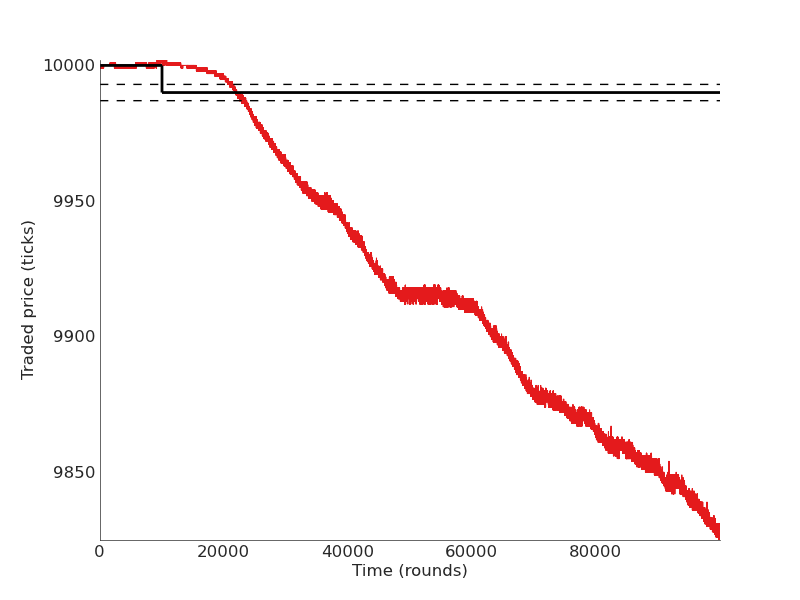
\includegraphics[width=0.5\textwidth]{manually_selected/crashes/shouganai.png}}
	\subcaptionbox{}
     [0.49\linewidth]{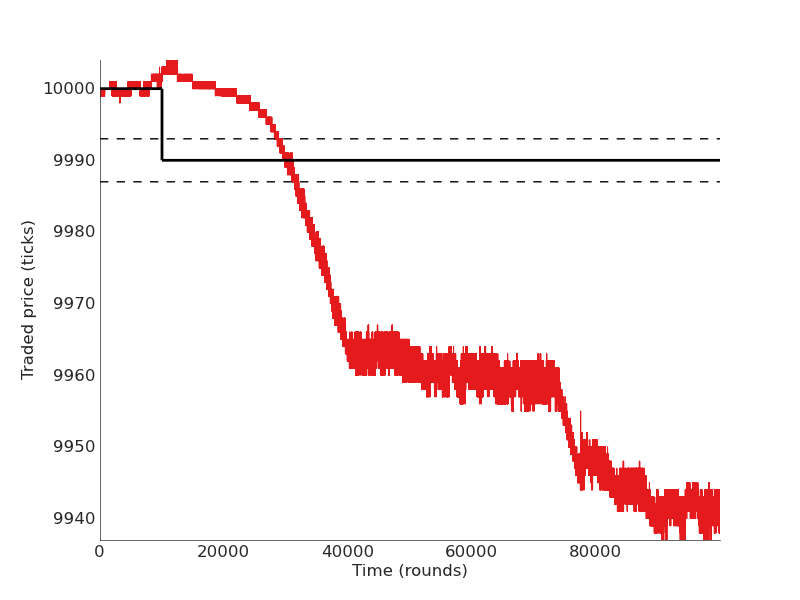
\includegraphics[width=0.5\textwidth]{manually_selected/crashes/slow_but_crash.png}}  
     \caption{Two examples of market crashes}
     \label{}
\end{figure}

\subsection{Frequency of crashes}

Crashes did not occur often particularly. Even during experiment \deleven, in which the genetic algorithm ended up prioritizing the market response times, and generate a large number of genes with many chartists and very fast market makers, the market had an overshoot of over 25 tick in just less than 0.2\% of the cases\footnote{The simulation was run around $4\cdot 10^5$ times, and 7989 of these had $\overshoot > 25$}. In experiment \dten, not a single case of markets with an overshoot of over 17 ticks was generated. 

XXX ADD A SMALL DISCUSSION OF HOW OFTEN CRASHES OCCUR IN REAL MARKETS

\subsection{Agent speed and market crashes}
XXX INSERT DATA THAT SHOWS THAT CRASHING MARKETS HAD FASTER AGENTS THAN NON CRASHING MARKETS


\section{Market makers causing the stock to be over-valued }
XXX NOT FINISHED. COLLECT EVIDENCE
This temporary over-evaluation of the assert is on the expense of Hence, the 

in \cite{}, the authors discussed the scenario in which a disparity between the this scenario and 


\section{title}
XXX discuss the variability of market behavior for markets simulated with the same parameters. is it reasonable that the same set of parameters can cause various types of behavior? XXX 


\section{Co-location}
Stable markets had an average market maker latency of $\ssmmlatencymu = 60 ms$, while crashing markets had an average of $\ssmmlatencymu = 30 ms$. Is it realistic that just a factor of two can have such a dramatic effect on the markets? 

The recent construction of the transatlantic fiber line reduced the latency from European markets to American markets 

Note also that latency is nt just a result of physical distance in the market. Network crowding can cause an increase in the latency as well. 


\section{Strategy crowding}
Strategy crowding is a commonly observed phenomenon in the field of multi-agent systems. XXX FIND REFERENCE XXX

\section{Future work}
A commonly used strategy among high frequency traders is that of arbitrage, 


